\section{Evaluation}

\begin{table}
    \centering
    \caption{Simulation parameters}\label{tab:params}
    \begin{tabular}{lrl}
        \toprule
        Parameter & Value & Clarification \\
        \midrule
        \# of steps & \num{100} & \\
        Repetitions & \num{100} & \\
        \glspl{RTT} & \( \left\{ 0.3, 0.6,\ldots,4.2 \right\} \) & \\
        \( \tau_\text{p} \) & \SI{250}{\milli\second} & Processing delay \\
        \( \tau_\text{c} \) & \( \text{\gls{RTT}} - \tau_\text{p} \) & Communication delay \\
        \( w_0 \) & \SI{1.0}{\second} & \\
        \( R_\text{min} \) & \SI{0.5}{\hertz} & Derived as \( R_\text{min} = {(2 w_0)}^{-1} \) \\
        \( \varphi \) & \num{1.5} & Scaling factor, \textcite{wang2019towards}\\
        \( P_0 \) & \SI{15}{\milli\watt} & Idle power \\
        \( P_\text{c} \) & \SI{45}{\milli\watt} & Communication power \\
        \( \alpha_\text{samples} \) & \( 1.9 \sigma^{-1} \) & For sample-count optimization. \\
        \( \beta_\text{samples} \) & \num{1.0} & For sample-count optimization. \\
        \( \alpha_\text{energy} \) & \( \tau_\text{c}(P_\text{c} - P_0) \) & For energy optimization. \\
        \( \beta_\text{energy} \) & \( P_0 \) & For energy optimization. \\
        \( \sigma \) & & \makecell[l]{Provided at runtime by\\a model of human timings.} \\
        \bottomrule
    \end{tabular}
\end{table}


In this section we evaluate the performance of our optimization framework and model of human behavior for the optimization of
\begin{enumerate*}[itemjoin*={{, and }}, itemjoin={{, }}]
    \item the number of samples captured
    \item the total energy consumption
\end{enumerate*}
per step in a \gls{WCA} task.
To this end, we introduce a simulated scenario within which we deploy two variants of our adaptive sampling approach as well as three reference sampling schemes.
Refer to \cref{tab:params} for the parameters used in the experimentation.

The scenario in question corresponds to a simulated execution of a \num{100}-step \gls{WCA} task.
To generate the execution times for each step in the task, we utilize an external model of human timings.
This model outputs an empirical distribution of execution times for each step according to the measured dynamic \glspl{TTF}, and we sample from this distribution to obtain individual execution time values.
The \glspl{RTT} for any inputs submitted to the \gls{WCA} during the task are constant during each repetition of the experiment, ranging from 0.3 to 4.2 seconds, with regular intervals. 
This range allows us to evaluate the performance of the approaches under different time constraints.

Within this scenario, we deploy two variants of our adaptive sampling approach as well as three reference sampling schemes.
We implement two variants of our framework for adaptive sampling
\begin{enumerate*}[itemjoin={{; }}, itemjoin*={{; and }}]
    \item a variant for optimizing for number of samples, based on \cref{eq:tnRayleigh:samples}, which we will refer to as the \emph{sample-count-optimized-aperiodic} approach
    \item a variant for optiminizing for energy consumption, based on \cref{eq:tnRayleigh:energy}, which we will refer to as the \emph{energy-optimized-aperiodic} approach
\end{enumerate*}.
We set the \( w_0 \) and \( \beta \) factors of our sample-count-optimized scheme to \SI{1.0}{\second} and \num{1.0}, respectively, for mathematical simplicity, and derive \( \alpha = 1.9 \sigma^{-1} \).
For the power constants used in the energy-optimized-aperiodic scheme, we reuse the values estimated by the authors in~\cite{moothedath2022energy1}, \( P_\text{c} = 45\,\si{\milli\watt} \) and \( P_\text{0} = 15\,\si{\milli\watt} \).
On the other hand, for the timing variables we define a constant processing delay \( \tau_\text{p} = 250\,\si{\milli\second} \) across all configurations and repetitions of the experiments; given then a constant \gls{RTT} for the task, we set \( \tau_\text{c} = \text{\gls{RTT}} - \tau_\text{p} \).

We utilize an internal, embedded model of human timings to provide updated values of \ensuremath{\sigma}.
This model utilizes an empirical distribution as output and is used for both the \emph{sample-count-optimized-aperiodic} and \emph{energy-optimized-aperiodic} sampling schemes.
Both the internal model of human timings used for the estimation of \ensuremath{\sigma} and the external model used for generating realistic execution times are parameterized with matching levels of neuroticism.
The neuroticism parameter can take on two values: low or high.
This ensures that the models are consistent in their behavior.

Additionally, we include implementations of three reference approaches.
The first of these corresponds to the heuristic, state-of-the-art adaptive sampling approach introduced in~\cite{wang2019towards}.
In this work, the authors introduce an adaptive sampling scheme for \gls{WCA} intended to reduce the number of samples processed per step while still meeting application responsiveness bounds.
At every sampling instant \( t \), the scheme adapts the sampling rate of the system according to the estimated likelihood of the user having finished the step.
They express this adaptive sampling rate \( R(t) \) as
\begin{equation}
    R(t) = R_\text{min} + \varphi\left( R_\text{max} - R_\text{min} \right) * CDF(t)
\end{equation}
\( R_\text{max} \) and \( R_\text{min} \) correspond to the maximum and minimum sampling rates of the system, respectively.
\( R_\text{max} \) can directly be assumed to correspond to \( 1 / \text{\gls{RTT}}_\mu \), where \( \text{\gls{RTT}}_\mu \) corresponds to the mean \gls{RTT} of the system.
\( R_\text{min} \) needs to either be calculated according to the latency bounds of the system or specified manually.
\( \varphi \) corresponds to a scaling factor and \( t \) to the time of the current sampling instant with respect to the start of the step.
\( CDF \) corresponds to the \gls{CDF} of a Gaussian distribution describing the execution times for the current step.
For our experimentation, we derive \( R_\text{min} \) from \( w_0 \).
As discussed previously, we assume that wait times are uniformly distributed between \SI{0}{\second} and sampling interval of each step.
A maximum expected wait time \( w_0 = 1.0\,\si{\second} \) thus translates into a maximum expected sampling interval of \SI{2.0}{\second}, yielding a minimum sampling rate \( R_\text{min} = {2.0\,\si{\second}}^{-1} = 0.5\,\si{\hertz} \).
% It should also be noted that in both aperiodic schemes, our sampling-count-optimized approach and the \gls{CDF}-based approach, there exists the possibility for sampling instants to be \emph{missed} due to the actual \gls{RTT} of the system being higher than the parameterization of the schemes.
% In these cases, both schemes will degrade into greedy sampling.

Finally, we introduce two reference sampling schemes representing best- and worst-case extremes.
The first of these corresponds to an offline optimum which uses an embedded \emph{oracle} to perfectly predict the execution time of each step.
Such an ideal scheme is thus able to always sample exactly once per step, with a constant wait time of zero.
The third and final reference scheme corresponds to one which \emph{greedily} samples as much as possible.
This represents a completely unoptimized design with no considerations for resource-consumption trade-offs; it simply attempts to maximize the number of captured samples per step.
This is an interesting approach to include as it corresponds to the sampling strategy used in most existing \gls{WCA} prototypes.

To ensure statistical significance, we repeat the \num{100}-step task scenario for each combination of \gls{RTT}, model neuroticism (low or high), and sampling scheme (sample-count-optimized-aperiodic, energy-optimized-aperiodic, state-of-the-art, offline optimum, or greedy) \num{100} times.
This repetition allows us to observe the performance trends across multiple iterations and obtain reliable statistical measures.

\subsection{Results}

\begin{figure*}
    \centering
    \begin{subfigure}[t]{\textwidth}
        \centering
        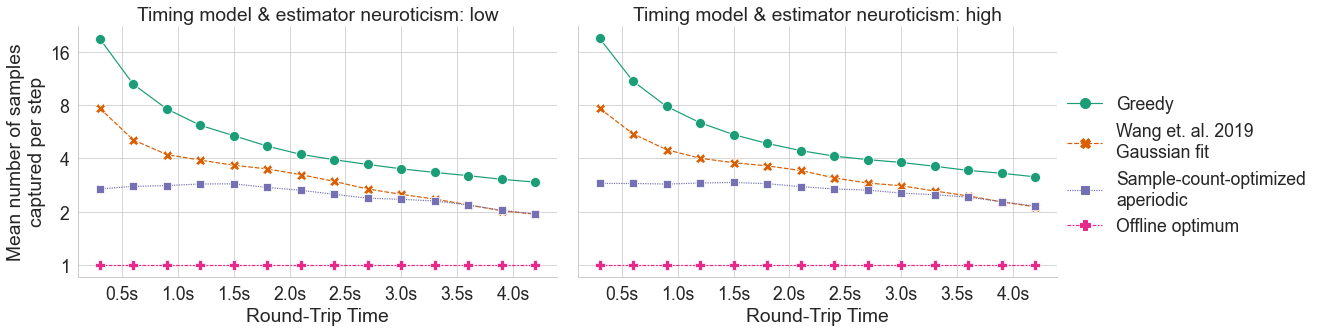
\includegraphics[width=\textwidth]{figs/new_model/sampling_optimization.png}
        \caption{%
            Round-trip time versus mean number of captured samples per step, averaged over all \num{100} repetitions of the experiment.
            Note the logarithmic scale on the vertical axis.
            Error bars indicate \SI{95}{\percent} \glspl{CI}.
        }
    \end{subfigure}\\
    \medskip
    \begin{subfigure}[t]{\textwidth}
        \centering
        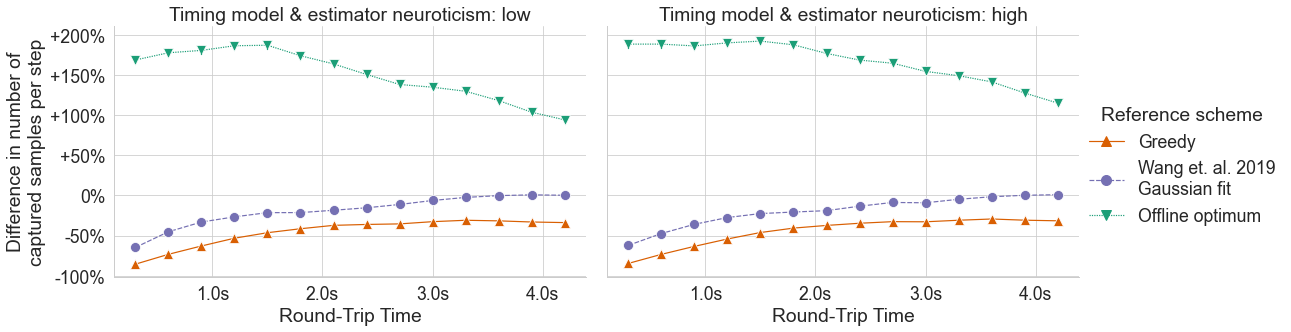
\includegraphics[width=\textwidth]{figs/new_model/sampling_optimization_diff.png}
        \caption{%
            Percentage difference in mean number of captured samples per step by the sample-count-optimized approach with respect to the three reference schemes.
            In other words, curves represent the relative performance of the sample-count-optimized scheme when using the corresponding reference scheme as baseline.
            Error bars indicate \SI{95}{\percent} \glspl{CI}, calculated using a two-sided t-test.
        }
    \end{subfigure}
    \caption{%
        Summary of results for experiment comparing the sample-count-optimized aperiodic sampling scheme to the reference schemes and \textcite{wang2019towards}'s \gls{CDF}-based approach.
    }\label{fig:optimization:samples}
\end{figure*}

The results of our investigation in the context of the optimization of number of samples per step are presented in \cref{fig:optimization:samples}.
These results clearly show the advantages of using the sample-count-optimized scheme over the current state-of-the-art.
The performance of \textcite{wang2019towards}'s approach appears to degrade with lower \glspl{RTT}, exponentially oversampling as latency tends to zero and the maximum sampling rate of the system tends to infinity.
On the other hand our sampling scheme consistently matches or beats the state-of-the-art while maintaining a relatively constant behavior with respect to \glspl{RTT}.
As mentioned above, the future feasibility and mass adoption of \gls{WCA} depends on these applications not hogging the available resources.
Our work advances this goal by being consistently more efficient than existing alternatives at minimizing the number of samples per step, and thus reducing network and processing load.

It should be noted that although both schemes seem to tend towards two samples per step as \glspl{RTT} increase, this is simply an artifact of our experimental setup.
As \glspl{RTT} increase above the expected wait time, the probability of the sum of the first sampling interval and the \gls{RTT} being larger than the execution time of the step tends towards \num{1.0}.
This leads to these sampling schemes consistently sampling only twice each step: a first sample which is taken before the execution time of the step, and a second one \gls{RTT} seconds later, after the execution time has been reached.

\begin{figure*}
    \centering
    \begin{subfigure}[t]{\textwidth}
        \centering
        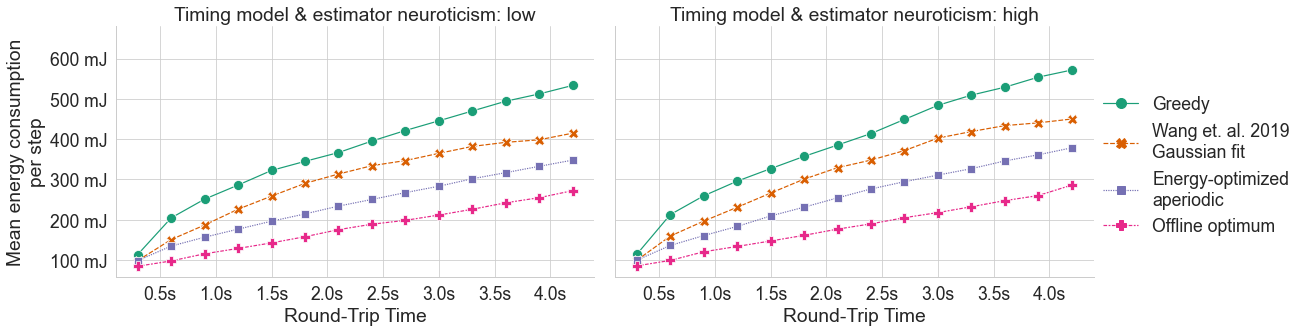
\includegraphics[width=\textwidth]{figs/new_model/energy_optimization.png}
        \caption{%
            Round-trip time versus mean per step energy consumption, averaged over all \num{100} repetitions of the experiment.
            Error bars indicate \SI{95}{\percent} \glspl{CI}.
        }
    \end{subfigure}\\
    \medskip
    \begin{subfigure}[t]{\textwidth}
        \centering
        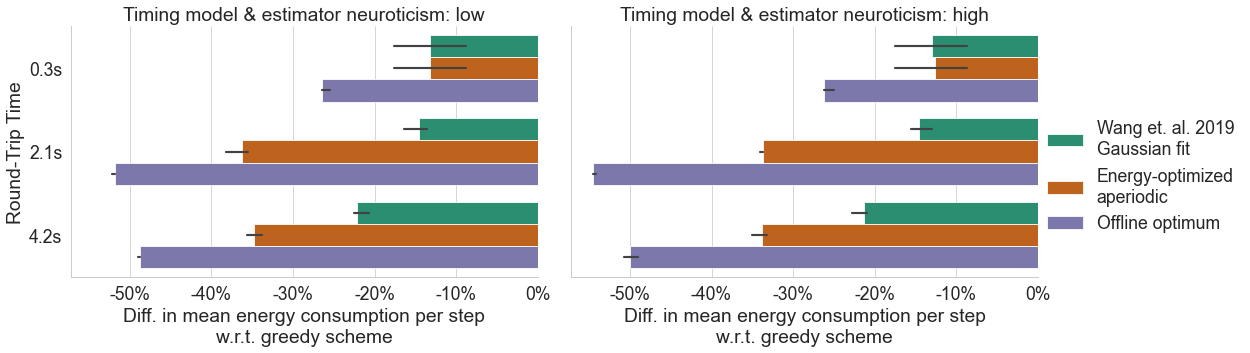
\includegraphics[width=\textwidth]{figs/new_model/energy_optimization_diff.png}
        \caption{%
            Percentage difference in mean per step energy consumption by the energy-optimized sampling scheme with respect to the three reference schemes.
            Error bars indicate \SI{95}{\percent} \glspl{CI}, calculated using a two-sided t-test.
        }
    \end{subfigure}
    \caption{%
        Summary of results for experiment comparing the energy-optimized aperiodic sampling scheme to the reference schemes and \textcite{wang2019towards}'s \gls{CDF}-based approach.
    }\label{fig:optimization:energy}
\end{figure*}

Likewise, \cref{fig:optimization:energy} showcases the advantages of our approach for the optimization of energy consumption in \gls{WCA}.
Our approach is consistently consumes \SI{20}{\percent} less energy than \textcite{wang2019towards}'s state-of-the-art, and is up to \SI{40}{\percent} more energy efficient than the greedy scheme.
Furthermore, once again the behavior of our approach is more consistent and reliable than the competition, exhibiting a flat curve of energy consumption much akin to that of the offline optimum in behavior.

\subsection{Implications of the model of human behavior for the study of \gls{WCA} footprints}\label{sec:implications:footprint}

\todo[inline]{This could potentially go in the discussion instead.}

In the following, we diverge from our main discussion regarding the implications of the optimization framework to briefly explore a implication of the model of human behavior itself on \gls{WCA} application lifetimes.
We will understand \emph{application lifetime} as the time it takes a user to complete a specified task.
This is an important metric for \gls{WCA} optimization, as it directly relates to system resource utilization and contention, and to energy consumption.

In order to illustrate the consequences of using a realistic model such as the one we describe in \cref{sec:model}, we introduce a much less complex and less realistic reference approach.
This reference model represents a naïve, first-order approximation to empirical execution time modeling, and consist simply of an \gls{exGaussian} distribution fitted to all execution time samples collected for~\cite{olguinmunoz2021impact}.
The \gls{exGaussian} \gls{PDF} has an ample body of research supporting its suitability for the modeling of the timing of human actions and reaction times~\cite{rohrer1994analysis,palmer2011what,marmolejo_ramos2022generalised}.

We begin by studying application lifetimes in a controlled, ideal setup by using the timing models to generate execution times for simulated sequences of \num{100} steps subject to constant \glspl{TTF}.
For each step, we feed the realistic model a predefined \gls{TTF} and obtain an \gls{exGaussian} distribution of execution times according to \cref{ssec:model:exectimes}.
This distribution is then randomly sampled obtain a single execution time for each step.
The first-order approximation described above is directly sampled instead.
We use the combination of \glspl{TTF} and execution times to calculate theoretical step duration times and subsequent total application lifetimes.
This is done for \num{25} linearly distributed \glspl{TTF} in the \SIrange[]{0}{5}{\second} range; \num{45} independent repetitions for each combination of model configuration and \gls{TTF}.

\begin{figure}
    \centering
    \begin{subfigure}[t]{.45\textwidth}
        \centering
        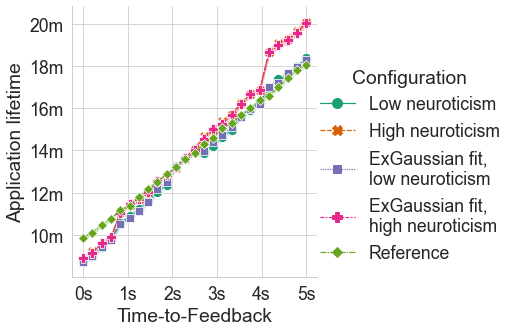
\includegraphics[width=\textwidth]{figs/new_model/lifetime_all_ttfs.png}
        \caption{%
            Evolution of mean application lifetimes as \glspl{TTF} increase.
            Error bars indicate \SI{95}{\percent} \glspl{CI}.
        }
    \end{subfigure}%
    \hfill%
    \begin{subfigure}[t]{.45\textwidth}
        \centering
        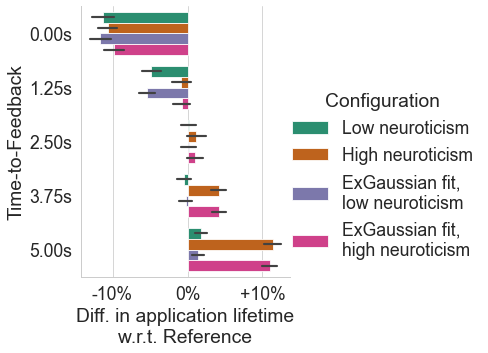
\includegraphics[width=\textwidth]{figs/new_model/lifetime_diff.png}
        \caption{%
            Percentage difference in mean application lifetimes with respect to the reference model at select \glspl{TTF}.
            Error bars indicate the \SI{95}{\percent} \glspl{CI}, calculated using a two-sided T-test.
        }
    \end{subfigure}
    \caption{\gls{TTF} versus application lifetime.}\label{fig:lifetimes}
\end{figure}

The results of this investigation are presented in \cref{fig:lifetimes}.
Compared to the reference model, our realistic model is, on average, roughly \SI{11}{\percent} faster when subject to low \glspl{TTF}.
At higher \glspl{TTF}, the behavior of the model depends on its level of normalized neuroticism.
At low neuroticism, the behavior of the realistic model results in total task durations that are basically indistinguishable from the reference model.
However, at high neuroticism, the model once again results in a considerable difference in total task duration with respect to the reference --- this time extending durations by \textasciitilde\SI{11}{\percent} on average.

\begin{figure*}
    \centering
    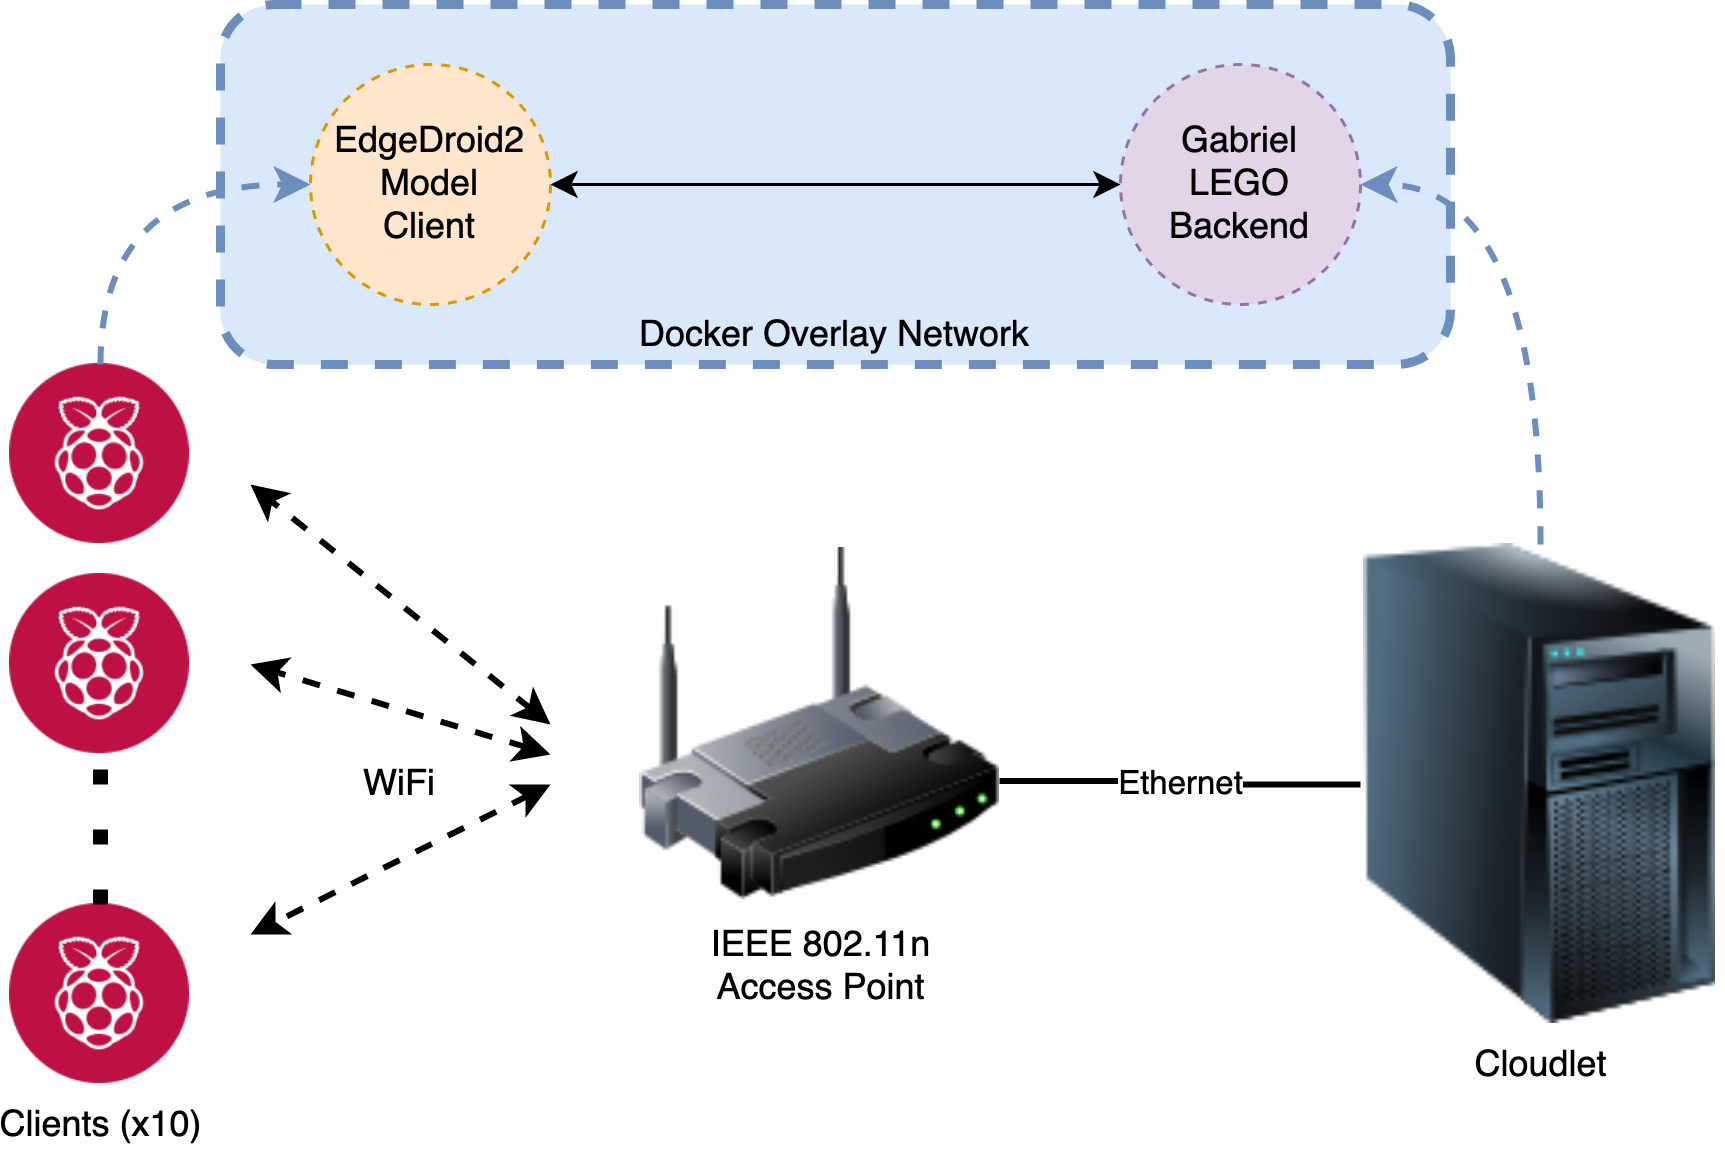
\includegraphics[width=.9\textwidth]{figs/EdgeDroid2ExperimentalSetup}
    \caption{%
        Experimental setup used to study the implications of the realistic models of human behavior for \gls{WCA}.
        We deploy containerized instances of the client-server loop running the models on a testbed consisting of \num{10} Raspberry Pi clients connected to a cloudlet over a \gls{COTS} \gls{IEEE} \num{802.11}b/g access point.
    }\label{fig:expsetup}
\end{figure*}

Next we study the effects of first- versus second-order models in a more realistic setting.
We integrate the execution time models (realistic and reference) with a custom Python3 client for the Gabriel \gls{WCA} platform~\cite{chen2018application}.
This custom includes a procedure for the generation of dynamic, synthetic traces of inputs from an existing trace.
It does so by greedily sampling from the existing video frames according to pre-calculated probabilities of specific types of frames (noisy, unfinished step, finished step, etc.) ocurring at particular instants in the task.
\todo[inline]{More details about the frames?}

These clients are then deployed on the Raspberry Pi clients of the testbed depicted in \cref{fig:expsetup}.
Instances of the Gabriel platform are deployed on the cloudlet.
Clients and cloudlet communicate over an \gls{IEEE} \num{802.11}b/g wireless network.
Our choice of wireless standard is simply motivated by a desire to amplify the potential effects of network congestion.

\begin{figure}
    \centering
    \begin{subfigure}[t]{.45\textwidth}
        \centering
        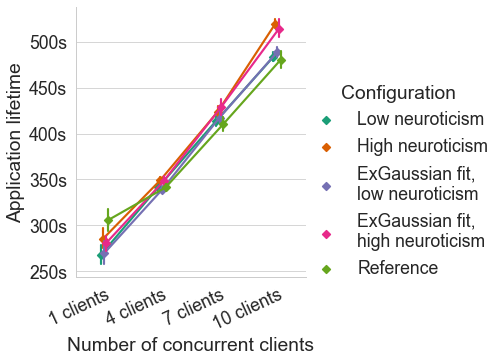
\includegraphics[width=\textwidth]{figs/new_model/lifetime_testbed}
        \caption{%
            Mean application lifetimes per testbed configuration.
            Note that due to the low number of samples, means have been calculated using the geometric instead of arithmetic average. 
            Error bars indicate \SI{95}{\percent} \glspl{CI}, calculated using bootstrapping.
        }
    \end{subfigure}%
    \hfill%
    \begin{subfigure}[t]{.45\textwidth}
        \centering
        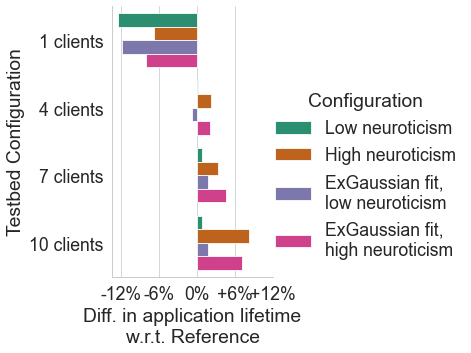
\includegraphics[width=\textwidth]{figs/new_model/lifetime_testbed_diff}
        \caption{%
            Percentage difference in mean application lifetimes with respect to the reference model.
            Confidence intervals have been omitted due to the low number of samples and the use of the geometric mean.
        }
    \end{subfigure}\\
    \bigskip
    \begin{subtable}{\columnwidth}
        \centering
        \begin{tabular}{lrrrr}
            \toprule
            \# clients & 1 & 4 & 7 & 10 \\
            \gls{RTT} & \SI{0.42}{\second} & \SI{1.12}{\second} & \SI{1.92}{\second} & \SI{2.68}{\second} \\
            \bottomrule
        \end{tabular}
        \caption{Mean measured \glspl{RTT} for each testbed configuration.}
    \end{subtable}
    \caption{Application lifetimes in the realistic scenarios.}\label{fig:testbed_lifetimes}
\end{figure}

We deploy configurations running \num{45}-step versions of the LEGO task described in~\cite{olguinmunoz2021impact}.
The testbed configurations include setups with \numlist{1;4;7;10} clients.
Each combination of testbed and timing model configuration is repeated \num{10} times.
The results are presented in \cref{fig:testbed_lifetimes}.
Owing to the low number of samples, specifically to minimize the effects of potential outliers, we opt here for the geometric rather than arithmetic mean to represent our results.
The results are nonetheless clear, and follow the same pattern as the previously discussed results under ideal, controlled circumstances.
With just a single client and mean \gls{RTT} of around \SI{400}{\milli\second}, all parameterizations of the realistic model achieved an average task duration \SIrange{6}{12}{\percent} shorter than the reference.
At \num{10} clients, the results mimic those at higher \glspl{TTF} in the ideal controlled setup, with high neuroticism parameterizations reaching \textasciitilde\SI{8}{\percent} longer application lifetimes.

These results highlight the importance of accurate execution time modeling when studying \gls{WCA} application lifetimes.
Not only do we see considerable differences in lifetimes at relatively moderate levels of system congestion, but the sign of these differences depends on the load placed on the system.
Imagine thus a system designer studying resource consumption optimization in a \gls{WCA}.
If they were to employ the reference model for their study on an unimpaired system, it could lead them to significantly underestimate the potential for optimization of resource consumption, leaving performance (and, potentially, monetary) gains on the table.
On the other hand, under heavy load, they would instead underestimate system resource occupation, again leading to performance losses.